\chapter{Project Development}

\section{Datasets}
There are several datasets on the internet, but none of them have the amount of sheer volume and actually useful data that is required for this task. The closest available was used, however, and it brought relatively acceptable levels of accuracy \citep{rf7}.
This dataset, paired with NLTK processing, stopwords and truncating words and verbs commonly used in the English language, was able to pinpoint if the user had a positive, neutral or a negative feeling in their input about 40\% of the time, approximately.
This is not really a good number for such a small amount of labels, but it's an improvement nonetheless. Previous versions with different approaches, combination of layers and datasets had less than 20\% of accuracy.

\section{Algorithm Used}
A standard LSTM algorithm was used with a softmax activation end layer. After much, much testing \textit{rmsprop} was chosen as the optimizer because of its slightly better results.
\begin{figure}[h]
	\centering
	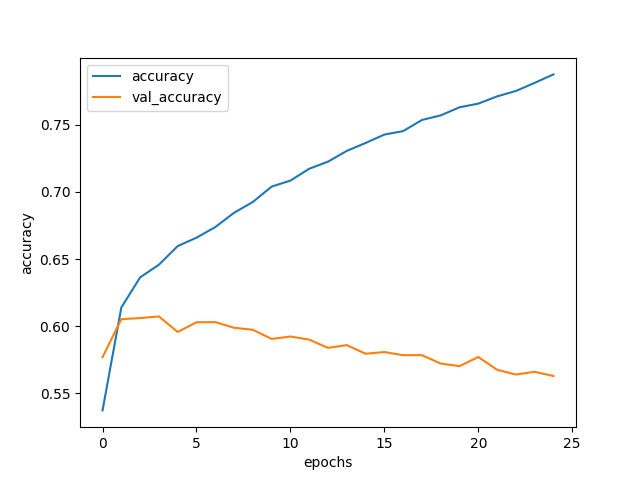
\includegraphics[scale=0.8]{Accuracy 2021-05}
	\caption{Accuracy Graph of the Algorithm Training}
	\label{fig:accuracy}
\end{figure}
\begin{figure}[h]
	\centering
	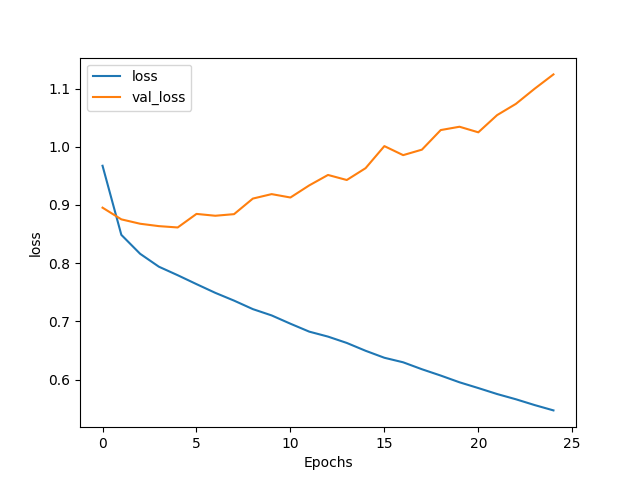
\includegraphics[scale=0.8]{Loss 2021-05}
	\caption{Loss Graph of the Algorithm Training}
	\label{fig:loss}
\end{figure}
\begin{figure}[h]
	\centering
	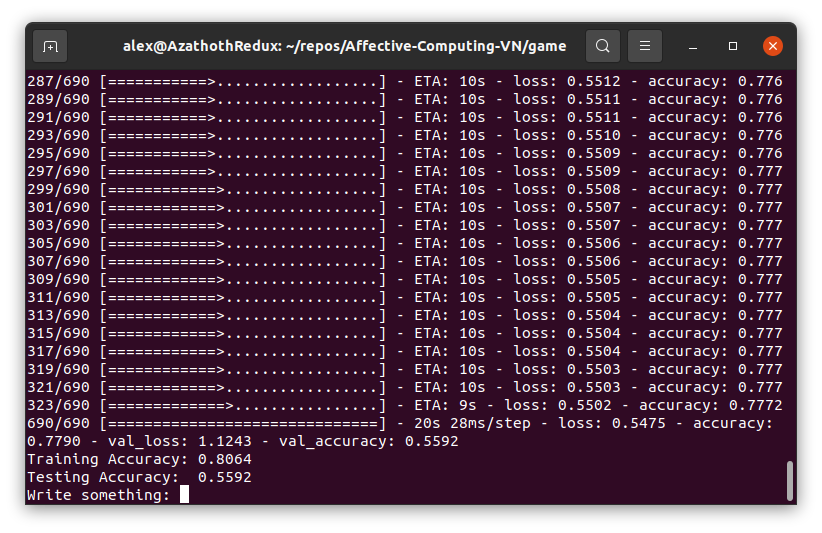
\includegraphics[scale=0.5]{Test 2021-05}
	\caption{Debugging of the Trained Model}
	\label{fig:test}
\end{figure}

\section{Interface}

